\documentclass[10pt,french,french]{article}
\usepackage{lmodern}
\usepackage{amssymb,amsmath}
\usepackage{ifxetex,ifluatex}
\usepackage{fixltx2e} % provides \textsubscript
\ifnum 0\ifxetex 1\fi\ifluatex 1\fi=0 % if pdftex
  \usepackage[T1]{fontenc}
  \usepackage[utf8]{inputenc}
\else % if luatex or xelatex
  \ifxetex
    \usepackage{mathspec}
    \usepackage{xltxtra,xunicode}
  \else
    \usepackage{fontspec}
  \fi
  \defaultfontfeatures{Mapping=tex-text,Scale=MatchLowercase}
  \newcommand{\euro}{€}
\fi
% use upquote if available, for straight quotes in verbatim environments
\IfFileExists{upquote.sty}{\usepackage{upquote}}{}
% use microtype if available
\IfFileExists{microtype.sty}{%
\usepackage{microtype}
\UseMicrotypeSet[protrusion]{basicmath} % disable protrusion for tt fonts
}{}
\usepackage[margin=0.80in]{geometry}
\ifxetex
  \usepackage{polyglossia}
  \setmainlanguage{}
\else
  \usepackage[shorthands=off,french]{babel}
\fi
\usepackage{longtable,booktabs}
\ifxetex
  \usepackage[setpagesize=false, % page size defined by xetex
              unicode=false, % unicode breaks when used with xetex
              xetex]{hyperref}
\else
  \usepackage[unicode=true]{hyperref}
\fi
\hypersetup{breaklinks=true,
            bookmarks=true,
            pdfauthor={},
            pdftitle={},
            colorlinks=true,
            citecolor=blue,
            urlcolor=blue,
            linkcolor=magenta,
            pdfborder={0 0 0}}
\urlstyle{same}  % don't use monospace font for urls
\setlength{\parindent}{0pt}
\setlength{\parskip}{6pt plus 2pt minus 1pt}
\setlength{\emergencystretch}{3em}  % prevent overfull lines
\setcounter{secnumdepth}{5}

\providecommand{\tightlist}{%
  %\setlength{\itemsep}{0pt}
  \setlength{\parskip}{0pt}
  }

%%% Use protect on footnotes to avoid problems with footnotes in titles
\let\rmarkdownfootnote\footnote%
\def\footnote{\protect\rmarkdownfootnote}


  \title{~\textsc{statistique bayésienne}\\
\hspace*{0.333em}Dating and forecasting turning point by Bayesian clustering with dynamic structure}
    \author{Romain Lesauvage et Alain Quartier-la-Tente}
    \date{}
  
\usepackage[T1]{fontenc}
\usepackage{caption}
\usepackage{graphicx}
\usepackage{natbib}
\usepackage[dvipsnames]{xcolor}
\usepackage{fontawesome5}
\DeclareMathOperator{\arctanh}{arctanh}
\usepackage{subcaption}
\usepackage{amsfonts}
\usepackage{dsfont}
\usepackage{bbold}
\usepackage{xspace}
\usepackage{enumitem}
\usepackage{pifont}
\usepackage{wrapfig}
\usepackage{textpos}
\usepackage{array}
\usepackage{multicol}


\usepackage[tikz]{bclogo}
\newcounter{comptEncadre}
\renewcommand\thecomptEncadre{%\thesection.
\arabic{comptEncadre}}
\definecolor{processblue}{cmyk}{0.96,0,0,0}
\newenvironment{encadre}[2][false]{\refstepcounter{comptEncadre}
      %\addcontentsline{exp}{encadres}{\protect\numberline{\thecomptEncadre}#1}%
\begin{bclogo}[couleur=processblue!5,arrondi=0.1,
logo=\bcloupe,barre=none,couleurBord=blue!60!green,nobreak = #1]{ {\sc \textbf{Encadré \thecomptEncadre}} -  #2}
\smallskip
}{\end{bclogo}}

\begin{document}

\maketitle


\begin{textblock*}{\textwidth}(0cm,-7.5cm)
\begin{center}

\includegraphics[height=2.5cm]{img/LOGO-ENSAE.png}
\end{center}
\end{textblock*}

\hypertarget{introduction}{%
\section{Introduction}\label{introduction}}

Dans son ouvrage \emph{Les vagues longues de la conjoncture}, Nikolai Kondratiev mettait en évidence l'existence de cycles économiques formés de deux périodes, une phase ascendante puis une phase descendante.
Bien que contestée et complétée par la suite par d'autres analyses, cette découverte des cycles économiques a très vite mené les chercheurs a essayé de savoir dans quelle phase l'économie se trouvait et, de fait, savoir déterminer et prévoir le moment le cycle s'inverse est un enjeu majeur.
C'est sur ce sujet que nous allons travaillé ici, à partir de l'article intitulé ``Dating and forecasting turning points by Bayesian clustering with dynamic structure: a suggestion with an application to Austrian data. Journal of Applied Econometrics'' \cite{Kaufmann}.

Ce papier poursuit un premier travail introduit par \cite{FruhwirthKaufmann}.
L'idée est de travail sur un ensemble de plusieurs séries temporelles que l'on va essayer de regrouper.
Nous chercherons à les regrouper au mieux afin d'étudier ensemble des séries qui possèdent la même dynamique.
Nous travaillerons alors sur deux périodes, selon que l'on est inférieur ou supérieur à la moyenne de croissance et on cherchera à déterminer le point de retournement dans le cycle.

Dans ce travail, nous commencerons par détailler les spécifications théoriques du modèle et l'estimation bayésienne associée.
Nous tenterons ensuite d'appliquer cette méthode à la manière de ce qui a été fait par \cite{Kaufmann} mais sur des données françaises.

\hypertarget{cadre-thuxe9orique}{%
\section{Cadre théorique}\label{cadre-thuxe9orique}}

\hypertarget{spuxe9cification-du-moduxe8le}{%
\subsection{Spécification du modèle}\label{spuxe9cification-du-moduxe8le}}

Dans la suite, nous travaillerons avec des séries centrées, réduites et corrigées des variations saisonnières.
Notons \(y_{it}\) la série correspondant à un taux de croissance, avec \(i \in \{1, \dots, N\}\) représentant les différentes séries à notre disposition et \(t \in \{1, \dots, T\}\) représentant les différentes périodes d'études.
Nous supposerons que nos séries suivent des processus autorégressifs, c'est-à-dire que l'on a \[ y_{it} = \mu_{I_{it}}^{i} + \phi_1^i y_{i,t-1} + \dots + \phi_p y_{i,t-p} + \epsilon_{it}\] avec \(\epsilon_{it} \sim \mathcal{N}\big(0, \displaystyle\frac{\sigma}{\lambda_i^2}\big)\).
L'indice \(I_{it}\) précisera à quel moment du cycle nous nous trouverons, ainsi on aura \(I_{it} \in \{1,2\}\).

Théoriquement, les séries étudiées sont supposées être indépendantes les unes des autres.
En pratique, cependant, il existe des séries qui suivent des évolutions proches et il peut donc être utile d'exploiter cette information pour notre estimation.
Nous allons donc chercher à créer des groupes de séries de manière intelligente.
Dans ce but, nous introduisons la variable \(S_i \in \{1, \dots, K \}\) qui indique dans quel groupe est classée la variable \(i\).
Dans la suite, nous supposons que toutes les séries d'un groupe vons avoir des paramètres distribués selon une même loi mais différente selon la position dans le cycle :

\[ \mu_{I_{S_i,t}}^i \sim \begin{cases}
\mathcal{N}(\mu_1^k,q_1^k) \text{ si } S_i = k \text{ et } I_{kt} = 1\\
\mathcal{N}(\mu_2^k,q_2^k) \text{ si } S_i = k \text{ et } I_{kt} = 2
\end{cases} \] \[ (\phi_1^i, \dots, \phi_p^i) \sim \mathcal{N}(\phi^k,Q_{\phi}^k) \text{ si } S_i = k\] Pour la suite, nous considérons que la période 1 (\(I_{kt} = 1\)) comme celle où l'on se trouve la croissance est supérieure à la moyenne (en haut du cycle) et la période 2 comme celle où la croissance est inférieure à la moyenne (en bas de cycle).
Nous ferons également l'hypothèse que \(I_{kt}\) suit un processus de Markov, c'est-à-dire \(\mathbb{P}(I_{k,t} = j | I_{k,t-1} = j) = \xi_{j,l}^k\) avec \(j,l \in \{1,2\}\).
Par propriété sur les chaînes de Markov, on sait donc que \(\forall j \in \{1,2\}, \sum\limits_{l=1}^2 \xi_{j,l}^k = 1\).
Cette spécification permet de repérer en temps réel les points où le cycle change de période.

Nous supposons que la variable \(S_i\) suit un modèle logit multinomial, c'est-à-dire \(\mathbb{P}(S_i = k |\gamma_1, \dots, \gamma_K, \gamma_{z,1}, \dots, \gamma_{z,K-1}) = \displaystyle\frac{\exp(\gamma_k + Z_k\gamma_{z,k})}{1 + \sum\limits_{l=1}^{K-1} \exp(\gamma_l + Z_l\gamma_{z,l})}\) où l'on prendra le groupe K comme référence (\(\gamma_K = \gamma_{z,K}=0\)), \(Z_i\) est un vecteur permettant de repérer l'appartenance à un groupe et les paramètres \(\gamma\) sont inconnus mais spécifiques aux groupes.

Enfin, il reste à ajouter une spécification pour en compte la dynamique du cycle.
Pour cela, nous supposons avoir deux groupes spécifiques pour la suite de l'analyse et \(K-2\) groupes indépendants.
Les séries telles que \(S_i = 2\) seront les séries qui mènent le cycle (indicateurs avancés), tandis que les séries pour lesquelles \(S_i = 1\) seront les séries qui coïncident avec le cycle (tels que le PIB).
Nous définissons donc une nouvelle variable \(I^*\) de la façon suivante: \[\begin{cases}
I^* = 1 := (I_{1t}=1,I_{2t}=1) \\
I^* = 2 := (I_{1t}=1,I_{2t}=2) \\
I^* = 3 := (I_{1t}=2,I_{2t}=1) \\
I^* = 4 := (I_{1t}=2,I_{2t}=2) 
\end{cases}\]

En cas d'incertitude sur la structure dynamique des nos séries, c'est-à-dire sur l'identification des groupes 1 et 2, on peut introduire un paramètre de structure \(\rho^*\), caractérisant la structure entre les groupes.
Il sera donc la réalisation d'une des \(K(K-1)\) permutations de \(\{1,2,0_{K-2}\}\).
On considéra que \(\rho^*=1\) pour le groupe des séries coïncidentes, \(\rho^*=2\) pour celles qui mènent le cycle, et toute autre valeur renverra aux séries aux comportements autonomes.

\hypertarget{estimation-bayuxe9sienne}{%
\subsection{Estimation bayésienne}\label{estimation-bayuxe9sienne}}

\hypertarget{notations}{%
\subsubsection{Notations}\label{notations}}

Dans la suite, notons \(\forall i \in \{1,\dots,N\}, y_i^t = \{y_{i,t},y_{i,t-1},\dots,y_{i,1}\}, Y_t = \{y_{1,t}, \dots, y_{N,t} \} \text{ et } Y^t = \{Y_t, \dots, Y_1\}\).
De même, notons \(S^N = \{S_1, \dots, S_N\}\) l'ensemble des indicatrices d'appartenances aux groupes, \(I^T = \{I_1^T, \dots, I_K^T\}\) où \(I_k^T=\{I_{k,T}, \dots, I_{k,1}\}\) les indicatrices d'états.
Enfin, nous notons \(\lambda^N = \{\lambda_1, \dots, \lambda_N\}\) qui regroupe les poids qui seront utilisés.

Par commodité, nous noterons également \(\theta=(\mu_1^1, \mu_2^1, \dots, \mu_1^K, \mu_2^K, \phi^1, \dots, \phi^K, Q^1, \dots, Q^K, \sigma^2, \xi^*, \xi^{\rho^*(k)=0},\gamma, \gamma_z)\) où \(Q^k = \begin{pmatrix} q_1^k & 0 & 0 \\ 0 & q_2^k & 0 \\ 0 & 0 & Q_{\phi}^k \end{pmatrix}\) représente l'hétérogénéité intra-groupe, \(\xi^{\rho^*(k)=0} = \{\xi_{11}^k,\xi_{12}^k,\xi_{21}^k,\xi_{22}^k\}\), \(\gamma = (\gamma_1, \dots, \gamma_{K-1})\) et \(\gamma_z = (\gamma_{z,1},\dots, \gamma_{z,K-1})\).

Nous pouvons passons à l'estimation par MCMC pour obtenir une posteriori sur le paramètre \(\psi = (\theta,S^N,I^T,\lambda^N,\rho^*)\).

\hypertarget{estimation-par-mcmc}{%
\subsubsection{Estimation par MCMC}\label{estimation-par-mcmc}}

Nous partons de \(\pi(\psi|Y^T) \propto L(Y^T|\psi)\pi(\psi)\) où \(L(Y^T|\psi)\) est la vraisemblance, que l'on peut réécrire.
En effet, \(L(Y^T|\psi) = \prod\limits_{t=p+1}^T\prod\limits_{i=1}^Nf(y_{i,t}|y_i^{t-1},\mu_{I_{S_i,t}}^{S_i},\phi^{S_i},Q^{S_i},\lambda_i,\sigma^2)\), avec \[f(y_{i,t}|y_i^{t-1},\mu_{I_{S_i,t}}^{S_i},\phi^{S_i},Q^{S_i},\lambda_i,\sigma^2)=\displaystyle\frac{1}{\sqrt{2\pi\nu_{it}^{S_i}}}\exp\big( -\displaystyle\frac{1}{2\nu_{it}^{S_i}}\big(y_{it} - \mu_{I_{S_i,t}}^{S_i} - \sum\limits_{j=1}^p \phi_j^{S_i}y_{i,t-1} \big)^2\big)\] Avec \(y_{it} = X^{S_i}_{it}\beta^{S_i} + \epsilon_{it}^*, \text{ où } \epsilon_{it}^*\sim N(0,\nu_{it}^{S_i}), X^{S_i}_{it} = (D_{1t}^{I(S_i)},D_{2t}^{I(S_i)},y_{i,t-1}, \dots, y_{i,t-p}),D_{jt}^{I(S_i)}=\mathbb{1}(I_{S_i,t}=j), \beta^{S_i} = (\mu_1^{S_i},\mu_2^{S_i}, \phi^{S_i}).\), et \(\nu_{it}^{S_i} = X^{S_i}_{it}Q^{S_i}X^{S_i'}_{it} + \displaystyle\frac{\sigma^2}{\lambda_i}\).

Nous supposerons dans la suite que la structure \(\rho^*\) est connue (déterminée par d'autres méthodes), nous pouvons alors réécrire la distribution a priori sur \(\phi\) ainsi :

\[\pi(\phi) = \pi(I^{*T}|\rho^*, \xi^*) \prod \limits_{\rho^*(k)=0} \pi(I^{T}_k|\rho^*,\xi^*)\pi(S^N|\gamma, \gamma_z,Z^N)\pi(\lambda^N)\pi(\theta)\]

où les densités \(\pi(I^{*T}|\rho^*, \xi^*)\),\(\pi(I^{T}_k|\rho^*,\xi^*)\) et \(\pi(S^N|\gamma, \gamma_z,Z^N)\) sont connues.
Nous supposerons que les poids (\(\lambda^N\)) sont indépendants et suivent une loi de Gamma.
Il reste à spécifier l'a priori sur \(\pi(\theta)\) : pour cela, nous décomposons \(\theta\) en blocs sur lesquels nous faisons des a priori standards.

Nous cherchons ensuite à générer à partir de la loi a posteriori \(\pi(\phi|Y^T)\), en se basant sur le procédé détaillé dans \cite{FruhwirthKaufmann}.
Nous pouvons raisonner en 4 étapes différentes :

\begin{enumerate}
\def\labelenumi{\arabic{enumi}.}
\item
  \(\pi(S^N|Y^T, I^T, \rho^*, \lambda^N, \theta)\)
\item
  \(\pi(I^T|Y^T, S^N, \rho^*, \lambda^N, \theta)\)
\item
  \(\pi(\lambda^N|Y^T, I^T, S^N, \theta)\)
\item
  \(\pi(\theta|Y^T,S^N,I^T)\)
\end{enumerate}

Dans la première étape, nous générerons les indicatrices de groupes pour chaque série puis, à partir de \(\rho^*\), nous obtenons une réalisation pour l'indicatrice d'état de l'étape 2.
Dans l'étape 4, toutes les distributions a posteriori sont conjugées aux a priori, sauf pour \(\gamma\) et \(\gamma_z\), nous utiliserons alors l'aglorithme de Metropolis-Hastings pour générer selon leur loi.

\hypertarget{application-aux-donnuxe9es-franuxe7aises}{%
\section{Application aux données françaises}\label{application-aux-donnuxe9es-franuxe7aises}}

L'article \cite{Kaufmann} a utilisé la spécification théorique présentée dans la partie précédente sur des données autrichiennes.
Nous avons décidé dans le cadre de ce travail d'appliquer cela sur des données françaises.
Nous avons donc récupéré un certain nombre de données liées au PIB ou aux enquêtes conjonctures\footnote{Nous avons décidé de ne retenir que les soldes d'opinion utilisés pour construire l'indicateur de retournement France publié par l'Insee (voir section \ref{sec:indretFr}) en supposant que, pour sa construction, les soldes les plus pertinents pour détecter les points de retournement avaient été retenus par l'Insee.
  Nous avons également retenu deux indicateurs synthétiques publiés par l'Insee : le climat des affaires France, qui retrace le cycle conjoncturel, et le climat de l'emploi France, qui retrace le cycle conjoncturel spécifique de l'emploi salarié.}, dont le détail est expliqué dans le tableau \ref{tableau_var}.

Nous avons retenu ici \(K=2\) groupes pour les séries : celles qui coïncident avec le cycle (\(S_i = 1\)) et celles qui le mène (\(S_i = 2\)).
Pour l'analyse, nous nous limitons aux hypothèses suivantes :

\begin{enumerate}
\def\labelenumi{\arabic{enumi}.}
\item
  La structure (\(\rho^*\)) est connue en avance : nous avons réparti chaque série dans un des groupes.
\item
  La classification est totale : on suppose qu'il n'y a pas de groupes de séries indépendantes.
\item
  L'\emph{a priori} sur \(S_i\) est de type logit.
\end{enumerate}

Nous avons adapté les programmes de \cite{Kaufmann} à nos données et nous analysons dans ce rapport les résultats obtenus.

Le modèle étudié ici se caractérise entre autres par la prise en compte de la spécification de l'hétérogénéité entre séries.
Ceci est illustré par le graphique \ref{heterogeneite}.
La figure \ref{fig:heterogeneite1} représente la moyenne de la somme des paramètres autorégressifs.
Dans l'article de \cite{Kaufmann}, l'importance de la prise en compte de l'hétérogénité était observée, ce qui semble s'observer sur les données française.
La figure \ref{fig:heterogeneite2} représente la moyenne des variances \(\frac{\sigma^2}{\lambda_i}\).
Cette fois-ci, on note une différence avec ce que donnaient les données autrichiennes.
En effet, notre distribution est plus étirée et plus applatie que celle de l'article.
Cela montre que la dispersion de l'erreur de variance est plus faible, ce qui s'explique sans doute par le processus de standardisation des séries préalables et par le fait que nous travaillons sur moins de séries.
Le graphique \ref{etats} représente la moyenne inconditionnelle de chaque groupe de série dans les deux états, selon qu'ils sont en-dessous de la croissance moyenne ou au-dessus.
Cela permet d'illustrer que, contrairement à l'article, nos deux groupes de séries n'ont pas exactement le même comportement puisque les séries sont décalées les unes par rapport aux autres.

\begin{figure}
\subfloat[Somme des coefficients de l'AR.\label{fig:heterogeneite1}]{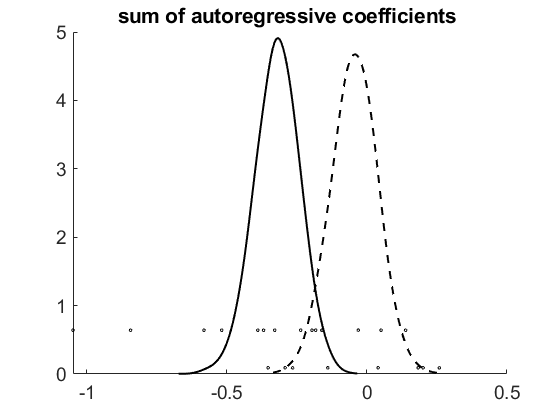
\includegraphics[width=8cm]{img/fig2a.png}}
\subfloat[$\sigma^2, \sigma^2/\lambda_i$.\label{fig:heterogeneite2}]{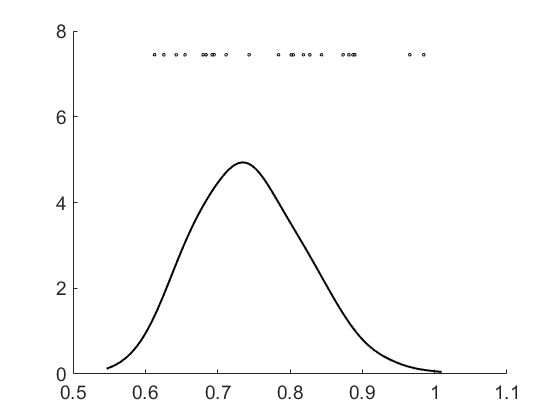
\includegraphics[width=8cm]{img/fig2b.png}}
\caption{Hétérogénéité des séries - groupe 1 (trait plein) et 2 (pointillés).}
\label{heterogeneite}
\end{figure}

\begin{figure}
\begin{minipage}{.5\textwidth}
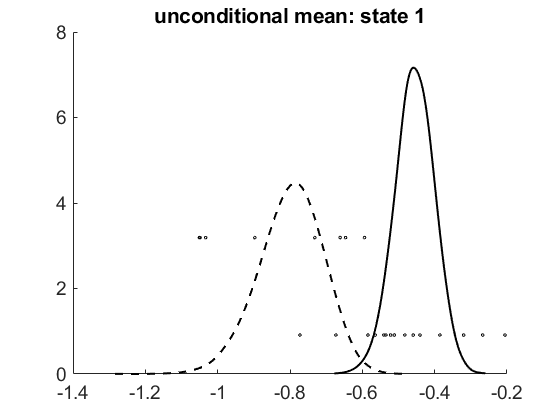
\includegraphics[width=8cm]{img/fig3b.png}
\end{minipage}
\hfill
\begin{minipage}{.5\textwidth}
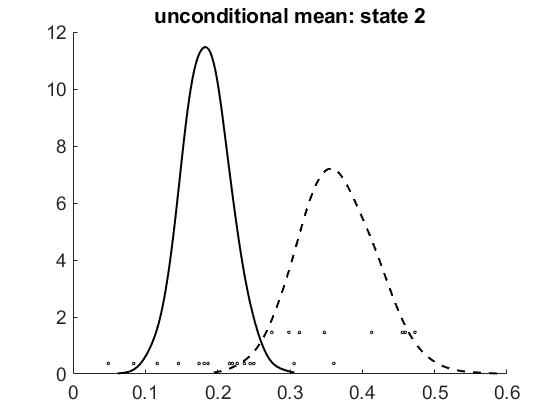
\includegraphics[width=8cm]{img/fig3a.png}
\end{minipage}
\caption{Moyenne inconditionnelle dans les différents états.}
\label{etats}
\end{figure}

Le graphique \ref{pi-gamma} permet de juger la significativité de l'information \emph{a priori} utilisée pour la classification.
Nous obtenons des conclusions légèrement différentes de celles de l'article : pour le groupe 1, la distribution \emph{a posteriori} des effets du PIB est éloignée de zéro, tandis que pour le groupe 2, on n'observe cela que pour les carnets de commandes (variable manuf-oscd).
Cela s'explique par la façon dont la classification \emph{a priori} a été effectuée, selon que la série allait être en avance ou non sur le PIB.

\begin{figure}
\centering
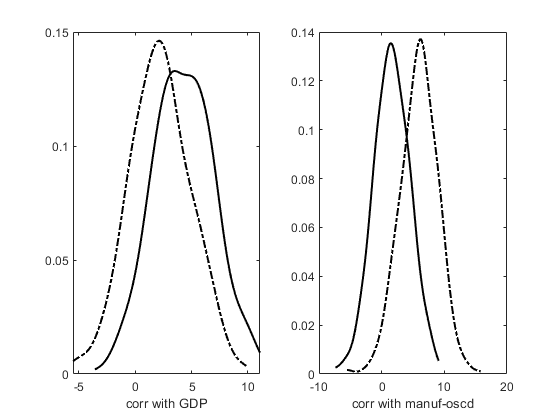
\includegraphics[width=12cm]{img/fig4.png}
\caption{$\pi(\gamma,\gamma_z|Y^T)$ - groupe 1 (trait plein) et 2 (pointillé).}
\label{pi-gamma}
\end{figure}

\begin{figure}
\begin{minipage}{.5\textwidth}
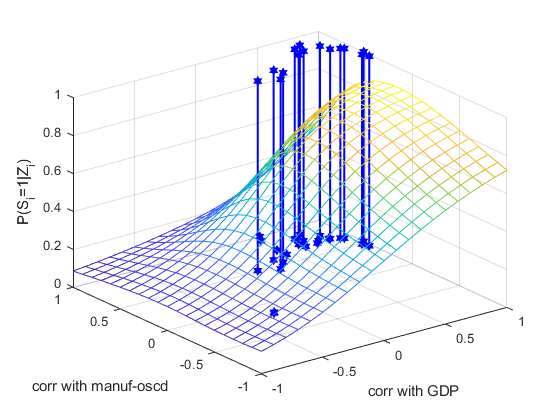
\includegraphics[width=8cm]{img/fig5a.png}
\end{minipage}
\hfill
\begin{minipage}{.5\textwidth}
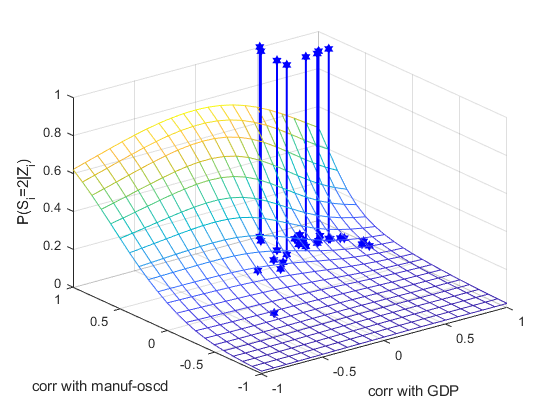
\includegraphics[width=8cm]{img/fig5b.png}
\end{minipage}
\caption{Probabilités \textit{a priori} et \textit{a posteriori} $P(S = j|Z,Y^T)$ et $P(S_i = j|Z_i,Y^T)$.}
\label{graph3d}
\end{figure}

Le graphique \ref{graph3d} permet de se rendre compte de l'effet de la corrélation avec le PIB et le carnet de commandes entre les groupes 1 (à gauche) et 2 (à droite).
La courbe représente \(P(S = j|Z,Y^T) = \int P(S=j|Z,\gamma,\gamma_z)\pi(\gamma,\gamma_z|Y^T)\mathrm{d}\gamma\mathrm{d}\gamma_z\), la probabilité conditionnelle sur le PIB et le carnet de commande.
Cette probabilité est la plus élevée pour les séries du groupe 1 qui sont fortement corrélées avec le PIB et corrélées positivement avec le carnet de commande, la corrélation avec le PIB semblant jouer un rôle plus important puisque la probabilité varie plus selon la valeur de cette dernière.
Nous retrouvons ici la définition du premier groupe de variables qui contient celles qui sont coincidentes avec le cycle et donc corrélées avec le PIB.
Pour le groupe 2, la valeur de la probabilité est maximale pour les séries fortement corrélées avec le carnet de commandes et cette variable semble être plus importante.
Cela conforte les analyses tirées du graphique \ref{pi-gamma}.

La hauteur des lignes verticales du graphique \ref{graph3d} représente la probabilité \(P(S_i = j|Z_i,Y^T)\) a posteriori pour une série d'appartenir aux groupes 1 et 2.
On remarque que dans la grande majorité des cas, cette probabilité a été mise à jour à 0 ou à 1, grâce à l'information supplémentaire obtenue.
On peut vérifier la qualité de notre pré-classification grâce à cela : elle semble cohérente.

\begin{figure}
\centering
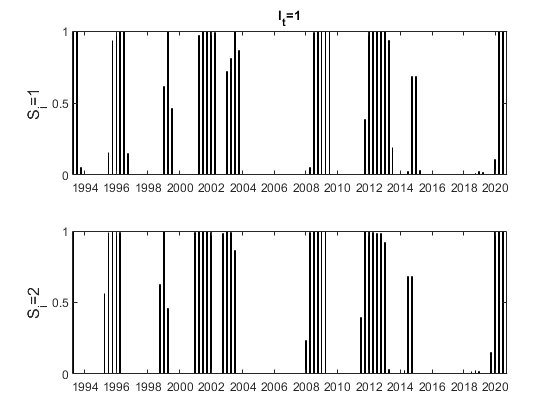
\includegraphics[width=15cm]{img/fig6.png}
\caption{Probabilités \textit{a posteriori} $P(I_{kt}=1|Y^T)$ des séries coïncidantes $(S_i=1)$ et qui mènent le cycle $(S_i=2)$ sur la période 1992-2020 avec une classification a priori.}
\label{retournements}
\end{figure}

Le graphique \ref{retournements} est central puisqu'il epermet de repérer les points de retournement de notre cycle.
Il représente les probabilités \(P(I_{k,t} = 1|Y^T)\) pour les séries des deux groupes, obtenues en moyennant les résultats sur \(M\) simulations.
On remarque que les résultats semblent significatifs puisque les probabilités ont des valeurs très proches de 0 ou de 1 dans une majorité de cas.
À partir de ce graphique, on définit le temps \(t\) comme un point de retournement si \(P(I_{k,t-1} = 1, I_{k,t} = 1 | Y^T) < 0,5\) et \(P(I_{k,t+1} = 1, I_{k,t+2} = 1 | Y^T) > 0,5\), c'est-à-dire une faible probalité de ne pas changer d'état à ce moment et, une fois qu'on a passé ce moment, une forte probabilité de rester dans le même état.
On peut donc repérer ici différents points de retournement qui correspondent à des réels évènements sur les marchés financiers en 1996 et 1999 (crise financière asiatique), 2002 et 2003 (krach boursier), 2009 (crise économique mondiale) ou encore 2013 (fin de la crise de 2008 avec encore des répercutions en France).
Une fois des données disponibles pour la période entière du Covid-19, il sera intéressant de voir ce qui a été capté par notre modèle.

\hypertarget{discussion}{%
\section{Discussion}\label{discussion}}

\hypertarget{pruxe9vision}{%
\subsection{Prévision}\label{pruxe9vision}}

Nous l'avons vu, notre modèle permet de repérer les points de retournement de l'économie.
Cependant, s'il est toujours intéressant de pouvoir le remarquer après coup, une utilisation plus immédiate serait appréciée.
Le modèle permet cela puisqu'il peut être utilisé dans une optique de prévision.
L'idée est d'utiliser la densité prédictive \emph{a posteriori} \(\pi(I^*_{T+h}|Y^T) = \pi(I^*_{T+h|T})\) et de simuler récursivement les valeurs futures à partir de cela.
En moyennisant nos résultats sur un grand nombre de simulations, on peut alors déterminer la probabilité d'être dans les différents états.

\hypertarget{sec:indretFr}{%
\subsection{Comparaison avec l'indicateur de retournement de l'Insee}\label{sec:indretFr}}

Afin de pouvoir juger de l'efficacité de notre modèle, il peut être intéressant de le comparer à des méthodes déjà existantes et utilisées par les instituts nationaux de statistiques.
En France, l'Insee publie un indicateur de retournement de conjoncture estimé à partir d'un modèle markovien à variables cachées sur des soldes d'opinion recodés en deux modalités (voir \cite{indretFR}).

La valeur de cet indicateur correspond à la différence entre la probabilité que la phase conjoncturelle soit favorable et la probabilité qu'elle soit défavorable.
Il évolue donc entre \(+1\) et \(-1\) : un point très proche de \(+1\) (respectivement de \(-1\)) signale que l'activité économique est en période de nette accélération (respectivement de nette décélération).
Les moments où l'indicateur est proche de 0 sont assimilés à des phases de stabilisation, c'est-à-dire de retour du rythme de croissance de l'activité vers sa moyenne de long terme.

Pour juger de la pertinence de la détection des points de retournement, il est nécessaire de disposer d'une datation des cycles d'expansion ou de contraction de l'activité.
Pour avoir une datation de référence, nous appliquons la méthode décrite par \cite{bardaji} : à partir du PIB trimestriel en volume, nous extrayon la composante cyclique de la série autour de sa tendance grâce à un filtre de Christiano-Fitzgerald en retenant des cycles d'une durée de 1,5 à 10 ans et une règle de censure pour éliminer les phases de moins de 4 trimestre.
Cela permet de déterminer les phases de ralentissement et d'accélération du PIB par rapport à sa tendance.
Les comptes nationaux étant encore provisoires à partir de 2018, la datation l'est également à partir de cette date.

\begin{figure}[h]
{\centering
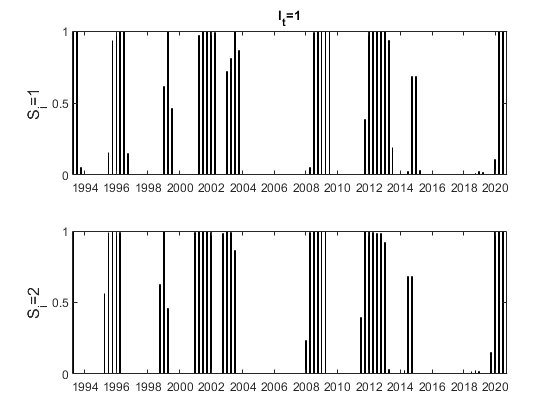
\includegraphics[height=8cm]{img/fig6.png}
\caption{L’indicateur de retournement France, la datation des cycles de croissance et points de retournement déterminés par approche bayésienne.}\label{fig:indret}}
\footnotesize
Lecture : l’indicateur de retournement (courbe) est en zone favorable quand il est proche de 1, défavorable quand il est proche de -1. Il est ici confronté à une datation de référence des cycles de croissance : les zones grises correspondent à un ralentissement du PIB (par rapport à sa tendance) et les zones blanches à une accélération.
\end{figure}

Le graphique \ref{fig:indret}\ldots.

\hypertarget{conclusion}{%
\section{Conclusion}\label{conclusion}}

TODO.

\newpage

\hypertarget{annexes}{%
\section{Annexes}\label{annexes}}

\begin{table}[h]{\centering
   \begin{tabular}{ | c | l | c|}
     \hline
     \textbf{Variable} & \textbf{Commentaire} & $S_i$ \\ \hline
     YER & PIB & 1\\ \hline
     MTR & Imports & 1 \\ \hline
     PCR & Consommation & 1\\ \hline
     ITR & Investissements & 1 \\ \hline
     XTR & Exports & 1 \\ \hline
     manuf-oscd & Enquête de conjoncture industrie -  carnet de commandes généraux & 2 \\ \hline
     manuf-oscde & Enquête de conjoncture industrie - carnet de commandes étrangers & 2 \\ \hline
     manuf-ossk & Enquête de conjoncture industrie - niveau des stocks de produits finis & 1\\ \hline
     manuf-tppre & Enquête de conjoncture industrie - tendance passée de production & 1\\ \hline
     manuf-tppre & Enquête de conjoncture industrie - tendance prévue de production & 2\\ \hline
     manuf-pgp & Enquête de conjoncture industrie - perspectives générales & 2\\ \hline
     ser-capa & Enquête de conjoncture services - évolution passée du chiffre d'affaires & 1\\ \hline
     ser-capre & Enquête de conjoncture services - évolution prévue du chiffre d'affaires & 2\\ \hline
     ser-dem & Enquête de conjoncture services - demande prévue  & 2\\ \hline
     bat-jcc & Enquête de conjoncture bâtiment - niveau des carnets de commandes & 2 \\ \hline
     bat-epa & Enquête de conjoncture bâtiment - évolutions passée des effectifs & 1\\ \hline
     bat-tuc & Enquête de conjoncture bâtiment - taux d'utilisation des capacités de production & 1\\ \hline
     bat-apa & Enquête de conjoncture bâtiment - évolution passée de l'activité & 1 \\ \hline
     bat-apre & Enquête de conjoncture bâtiment -  évolution prévue de l'activité & 2\\ \hline
     CLIMAT-FR & Climat des affaires France & 1 \\ \hline
     CLIMAT-FR-EMPL & Climat de l'emploi France  & 1 \\ \hline
     HIPC-FO & Indice des prix - nourriture & 1 \\ \hline
     HICP-IG & Indice des prix - produits industriels & 1 \\ \hline
     HICP-E & Indice des prix - énergie & 1 \\ \hline
     HICP & Indice des prix & 1 \\ \hline
     IPI-CZ & Indice de production industrielle - industrie manufacturière & 1 \\
     \hline
   \end{tabular}
   \caption{Variables utilisées dans l'analyse.}\label{tableau_var}}
  \footnotesize
Note de lecture : $S_i=1$...
\end{table}

\newpage

\nocite{*}

\begin{thebibliography}{999}
\bibitem[Sylvia Kaufmann (2010)]{Kaufmann} Kaufmann S. (2010). Dating and forecasting turning points by Bayesian clustering with dynamic structure: a suggestion with an application to Austrian data. Journal of Applied Econometrics, \textbf{25}(2): 309-344 
\bibitem[Frühwirth-Schnatter S, Kaufmann S. (2008)]{FruhwirthKaufmann} Frühwirth-Schnatter S, Kaufmann S. (2008). Model-based clustering of multiple time series. Journal of Business and Economic Statistics \textbf{26}(1): 78
\bibitem[Bortoli \emph{et al} (2015)]{indretFR} Bortoli C., Gorin Y., Olive P.-D. et Renne C. (2015), « De nouvelles avancées dans l’utilisation des enquêtes de conjoncture de l’Insee pour le diagnostic conjoncturel », \emph{Note de Conjoncture}, mars, p. 21-41.
\bibitem[Bardaji \emph{et al} (2009)]{bardaji} Bardaji J., Clavel L. et Tallet F.,(2009), « Constructing a Markov-Switching Turning Point Index Using Mixed Frequencies with an Application to French Business Survey Data », \emph{OECD Journal: Journal of Business Cycle Measurement and Analysis}, Vol. 2009/2.
\end{thebibliography}

\end{document}
